% UTF-8

% single-chapter commands
\documentclass[../main/thesis.tex]{subfiles}
\onlyinsubfile{\setcounter{chapter}{4}}  % single-chapter command
\onlyinsubfile{\pagenumbering{roman}\setcounter{figure}{40}}
\begin{document}


\chapter{Implementierung}
\label{ch:impl}

\section{Entwicklungsumgebung}
\label{ch:impl-env}

Zur Umsetzung der entwickelten Algorithmen in Software wurde die Plattform Java verwendet.
Die Wahl von Java erfolgte neben der Vertrautheit des Verfassers mit dem zugehörigen \term{framework} auch aufgrund zu erwartender Effizienzvorteile von kompiliertem Code gegenüber Skriptsprachen wie etwa Perl.
% einer Empfehlung der Geofabrik folgend

Java als imperative Sprache erlaubt es nicht, Algorithmen mit dem gleichen Grad an Abstraktion zu beschreiben wie zuvor in Kapitel~\ref{ch:algorithm-parts} geschehen.
Dort konnten zugunsten einer vereinfachten
% jedoch präzisen, cf. EWD656
Beschreibung praktische Erwägungen wie der Bedarf an Rechenzeit und Speicherplatz teilweise hintenanstehen.
Bei der Implementierung in Java sollten hingegen sorgfältig solche Datenstrukturen gewählt werden, die eine effiziente Ausführung erlauben, und die Algorithmen soweit nötig entsprechend angepasst werden.
Das Ergebnis wird in Abschnitt~\ref{ch:data-structures} beschrieben.

Während der Entwicklung wurde versucht, so viel existierenden Code in Form von \term{frameworks} und anderen Programmbibliotheken wiederzuverwenden wie möglich.
Diese Bestrebung verursachte Probleme, wie auch später in Abschnitt~\ref{ch:impl-io} dargelegt wird.
Bei der Entwicklung kamen zuletzt die folgenden Plattformen und Bibliotheken zum Einsatz:

\begin{itemize}[nosep]
	\item Mac OS X 10.11.6
	\item Java™ Standard Edition JDK 8 Update 162\\ \url{http://www.oracle.com/technetwork/java/javase/downloads/}
	\item Apache Ant 1.10.2 \quad \url{https://ant.apache.org/}
	\item args4j 2.33 \quad \url{http://args4j.kohsuke.org/}
	\item GeoTools 18.0 \quad \url{http://www.geotools.org/}
	\item TestNG 6.8 \quad \url{http://testng.org/}
	% http://web.archive.org/web/20121113133417/http://testng.org/testng-6.8.zip (all other releases appear to be corrupt; I'm probably doing something wrong)
	\item GDAL 2.2.2 \quad \url{http://www.gdal.org/}
\end{itemize}

Ursprünglich wurden ältere Softwareversionen verwendet.
Die nötigen Anpassungen an die hier genannten aktuellen Versionen waren gering, Kompatibilität mit den älteren Versionen ist jedoch gegenwärtig aufgrund von Änderungen in GeoTools nicht mehr vollständig gegeben.
Der Code ist dabei noch immer konform zur Syntax von Java 6. \cf{GJSB05}

Der folgende Abschnitt erläutert einige Überlegungen, die bei der Auswahl der Bibliotheken relevant waren.



\section{Systemarchitektur}
\label{ch:impl-architecture}

Für ein gut funktionierendes Gesamtpaket sind vor der Umsetzung von vorgegebenen Algorithmen in ausführbarem Code einige praktische Aspekte zu bedenken.

Da die entwickelten Algorithmen ein für das jeweilige Anwendungsgebiet optimiertes kartesisches Koordinatennetz verlangen (vgl. Abschnitt~\ref{ch:split-algorithm}), sind die aus der \osm-Datenbank stammenden Eingangsdaten nach Länge und Breite vor der Verarbeitung in einem geeigneten Kartennetzentwurf abzubilden.
Hierzu bietet sich unter anderem die UTM-Abbildung an \term{(Universal Transverse Mercator),} welche einen querachsigen Schnittzylinder winkeltreu abbildet und zur Minimierung des Maßstabsfehlers in jeweils 6° breite Zonen unterteilt. \cf[57--58]{Sny87}
Zur Vereinfachung wird die Implementierung zunächst auf eine einzelne UTM-Zone beschränkt.

Weiterhin stellt sich die Frage nach der Benutzerschnittstelle der Software.
Die gewählte Plattform Java bietet verschiedene Möglichkeiten, graphische Benutzeroberflächen (\term{graphical user interface,} GUI) zu gestalten.
Denkbar wäre beispielsweise eine Integration in den weit verbreiteten \osm-Editor JOSM als \term{plug-in.}
Das Entwickeln und Debuggen einer GUI-Anwendung wäre jedoch zeitaufwändig.
Ohnehin würde es ein modularer Aufbau der Anwendung erlauben, zu einem späteren Zeitpunkt eine optionale GUI zu ergänzen.
Aus diesen Gründen soll im Rahmen dieser Arbeit auf eine GUI zugunsten einer einfachen textbasierten Kommandozeilen-Schnittstelle (\term{command-line interface,} CLI) verzichtet werden.
Zum Parsen der CLI-Parameter bieten sich einfache Bibliotheken wie etwa args4j an.

Zur Verarbeitung beliebiger Geodaten müssen diese aus Datenspeichern eingelesen und wieder ausgegeben werden können.
Um Entwicklungszeit zu sparen, soll hierfür nach Möglichkeit ein existierendes \term{framework} genutzt werden.
%Zur Vermeidung einer zu engen Kopplung der Generalisierung an das gewählte \term{framework} sollte jedoch möglichst vermieden werden, die Primitiven des \term{frameworks} intern weiterzubenutzen.
%Stattdessen sollten eigene Datenstrukturen genutzt werden, um Modularität zu fördern.
%Die dabei entstehenden Kosten in Form von Rechenzeit und Speicherverbrauch sind zu berücksichtigen.

Die in Abschnitt~\ref{ch:split-algorithm} gegebene Definition für \textproc{NaheSegmente} kann leicht mit Hilfe eines R-Baums als räumlicher Index umgesetzt werden.
Die \textproc{Hülle} ist dabei das minimal umgebende Rechteck eines Blatts im R-Baum.
Nachdem die \osm-Eingangsdaten vor der Generalisierung vollständig bekannt und somit statisch sind, bietet sich der Einsatz eines gepackten R-Baums an \cf[255-256]{RSV02}.
Ein solcher Baum wird von der JTS Topology Suite (JTS) angeboten, welche vom \term{framework} GeoTools als Implementierung des Geometriemodells verwendet wird.

GeoTools bietet außerdem Möglichkeiten zur Ein- und Ausgabe (\term{input/output,} I/O) von Geodaten in zahlreichen Formaten einschließlich der Transformation von Koordinatensystemen.
Zwar wird das native \osm-XML-Format ebensowenig unterstützt wie das neuere Protocol Buffer Binary Format (PBF).
Das verbreitete Format ESRI~Shapefile wird jedoch unterstützt.
Die Geofabrik stellt aktuelle OSM-Auszüge öffentlich als Shapefile bereit.
Alternativ lassen sich Shapefiles leicht mit gängiger Software wie etwa GDAL aus anderen Formaten erzeugen.
GDAL ermöglicht dabei auch den Zuschnitt auf ein abgegrenztes Untersuchungsgebiet, was sich für Testzwecke anbietet.

\onefigure[12cm]{ht}{
	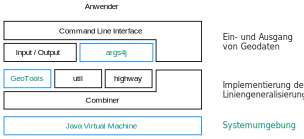
\includegraphics[width=\ScaleIfNeeded]{../chapter5/system-concept}
	\caption
		[Komponenten der entwickelten Software]
		{Komponenten der entwickelten Software (schwarz: eigene Entwicklung, blau: benutzte Bibliothek)}
	\label{fig:system-concept}
}

Zusammengesetzt ergibt sich aus den besprochenen Aspekten die in Abbildung~\ref{fig:system-concept} dargestellte Architektur:
Dem Anwender steht eine Kommandozeilen-Schnittstelle (CLI) zur Verfügung, welche die Bibliothek args4j zum Parsen der Parameter sowie selbst entwickelte Routinen zur Ein- und Ausgabe der Geodaten verwendet (welche ihrerseits auf GeoTools zurückgreifen).

Die CLI steuert damit die eigentliche Liniengeneralisierung (hier als \term{Combiner} bezeichnet), welche ihrerseits neben dem \term{framework} GeoTools noch einige selbst entwickelte Hilfsmodule verwendet, die nicht vom \term{Combiner} abhängig sind und deshalb als separates Softwarepaket dargestellt werden („util“).
Schließlich sitzt zwischen \term{Combiner} und CLI ein mit „highway“ bezeichnetes Paket, welches versucht, die Logik des in Abschnitt~\ref{ch:case-selection} ausgewählten Spezialfalls an einem einzigen Ort zu bündeln, um die Anpassung auf andere Spezialfälle zu erleichtern.

% Noch mal Modularisierung; java Packages erwähnen/erklären? -> eher nein

In den folgenden Abschnitten wird näher auf die Implementierung der Liniengeneralisierung insbesondere im \term{Combiner} eingegangen.



\section{Datenstrukturen}
\label{ch:data-structures}

% - übergeordnete Frage: warum _so_ und nicht anders?

Aus Gründen der Übersichtlichkeit werden in den folgenden Abschnitten nur wesentliche Aspekte und wichtige Entscheidungen behandelt.
Für Detailfragen sei auf die Dokumentation der Programmierschnittstelle verwiesen, welche in englischer Sprache als Teil der Softwareentwicklung im Javadoc-Format angelegt wurde und sowohl im Java-Quellcode als auch im HTML-Format zugänglich ist (\url{http://arne.johannessen.de/thesis}).

Anhang~\ref{appx:identifiers} löst Bezeichner aus Abschnitt~\ref{ch:algorithm-parts} zu Bezeichnern im Quellcode auf.



\subsection{Grundlegendes Geometrie-Modell von GeoTools}
\label{ch:data-structures-geotools}

Zur Umsetzung der in Abschnitt~\ref{ch:algorithm-parts} definierten geometrischen Algorithmen werden zunächst Strukturen zur Repräsentation der grundlegenden Datentypen benötigt.
Im Kontext dieses Projekts sind dies:
\begin{enumerate}[nosep]
	\item Punkt (\osm-\term{node})
	\item Segment (Verbindung von zwei Punkten als Teil eines Linienzugs)
	\item Linienzug (\osm-\term{way})
\end{enumerate}

\noindent
Das \term{framework} GeoTools benutzt dazu die JTS Topology Suite, die wie zuvor beschrieben ohnehin wegen des R-Baums für \textproc{NaheSegmente} zum Einsatz kommen soll.
JTS bietet mit der \code{Geometry}-Hierarchie Datenstrukturen nach ISO~19125\hbox{-}1 an, die grundsätzlich auch für die Implementierung der Algorithmen aus Abschnitt~\ref{ch:algorithm-parts} geeignet wären.
\cf{jts:geom}

Die Algorithmen \textproc{Splitten} und \textproc{Analyse} ordnen den Segmenten allerdings zusätzliche Attribute zu ($\relation{wurzel}$ bzw. $\relation{parallelLinks}$ / $\relation{parallelRechts}$).
Dies unterstützt JTS zwar in Form von \term{user data objects}.
% http://atetric.com/atetric/javadoc/com.vividsolutions/jts-core/1.14.0/com/vividsolutions/jts/geom/Geometry.html#getUserData--
Weil jedoch die Arbeit damit eher umständlich ist, wäre dies nur sinnvoll, wenn die Nutzung der JTS-Datenstrukturen andere Vorteile bietet.

Dies ist jedoch nicht der Fall.
Im Gegenteil passen die JTS-Datenstrukturen nicht gut auf die definierten Algorithmen:
Diese beschränken sich zu einem großen Teil auf Segmente aus exakt zwei Punkten, während JTS von längeren Linienzügen ausgeht.
Die Algorithmen machen sich außerdem zunutze, dass sich Segmente direkt als Vektoren interpretieren lassen (vergleiche Abschnitt~\ref{ch:split-algorithm}).
Routinen zur Vektor-Mathematik bietet JTS zwar grundsätzlich an, aber wichtige Teile davon sind nicht spezifiziert.
Beispielhaft sei die Klasse \code{jts.math.Vector2D} genannt, deren Methode \code{angle} offenbar Winkel berechnet, jedoch in keiner Weise dokumentiert ist.
\cf{jts:mathVector2D}
Die Definition der \textproc{Analyse} auf Parallelität verlangt jedoch einen bestimmten Wertebereich für Winkel von Vektoren.
Obwohl sich die derzeitige Implementierung von \code{angle} leicht anhand des Quellcodes von JTS ermitteln ließe, ist die Methode nicht zuverlässig verwendbar, weil ohne Dokumentation bereits unklar bleibt, ob die derzeitige Implementierung überhaupt korrekt ist.

Hinzu kommt, dass auch die von JTS angebotenen Operationen zur Manipulation geometrischer Daten -- abgesehen vom räumlichen Index -- hier wenig hilfreich sind.
Ein direktes Verwenden der bereitgestellten JTS-Datenstrukturen erscheint folglich insgesamt betrachtet nicht sinnvoll zu sein.
Stattdessen wurde ein eigenes Datenmodell entwickelt, das im Folgenden beschrieben wird.

JTS bietet die Möglichkeit, das \term{framework} zusammen mit eigenen Datenstrukturen zu benutzen, wenn diese bestimmte Schnittstellen anbieten.
\cf[11]{jts:devguide}
% z. B. CoordinateSequence
Dies käme hier durchaus in Betracht, damit die eigenen Datenstrukturen zukünftig von Dritten unmittelbar mit JTS genutzt werden können.
Beispielsweise könnten so zusammengefasste Linienzüge als Ergebnisse der hier entwickelten Software direkt mit JTS einer Formvereinfachung unterzogen werden.
Weil dies jedoch nicht Bestandteil dieser Arbeit ist und ein Implementieren jener Schnittstellen keinen direkten Nutzen hat, wurde darauf zunächst verzichtet.
Es ließe sich für eine zukünftige Version leicht ergänzen.



\subsection{Eigenes grundlegendes Geometrie-Modell}
\label{ch:data-structures-new}

Es erwies sich also als notwendig, auf dieser Basis ein neues Geometriemodell zu entwickeln.
Ein zusammengesetztes Diagramm des Ergebnisses ist Anhang~\ref{appx:fullpage-model} zu entnehmen.
Vereinfacht auf die grundlegenden Geometrie-Datentypen ergibt sich das in Abbildung~\ref{fig:impl-geometry-model} gezeigte Datenmodell.
Die \textproc{Segmente} sind -- wie in Abschnitt~\ref{ch:split-algorithm} beschrieben -- zunächst nicht in den Eingangsdaten vorhanden; sie daraus durch Segmentierung herzustellen, ist jedoch einfach.

%   https://de.wikipedia.org/wiki/Assoziation_(UML)#Aggregation_und_Komposition

\onefigure{ht}{
% [Dataset]1 <>-- 0…n[Line]1 <>-- 1…n[Segment]1…n <>-- 2[Node]
	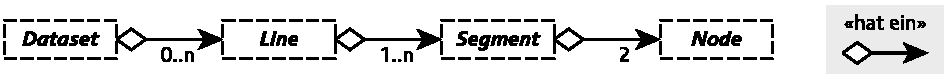
\includegraphics[scale=.8]{../chapter5/model-geometry}
	\caption{Datenmodell für die Geometrie}
	\label{fig:impl-geometry-model}
}

Die hier gezeigten Datentypen wurden als Interfaces (formale Schnittstellendefinitionen) umgesetzt, um ihre eventuelle Wiederverwendung zu erleichtern. \cf[18]{GHJV95}
Abbildung~\ref{fig:impl-class-structure-splitting} zeigt die bei der Implementierung dieses Datenmodells entstandene Klassenstruktur.

\onefigure{ht}{
	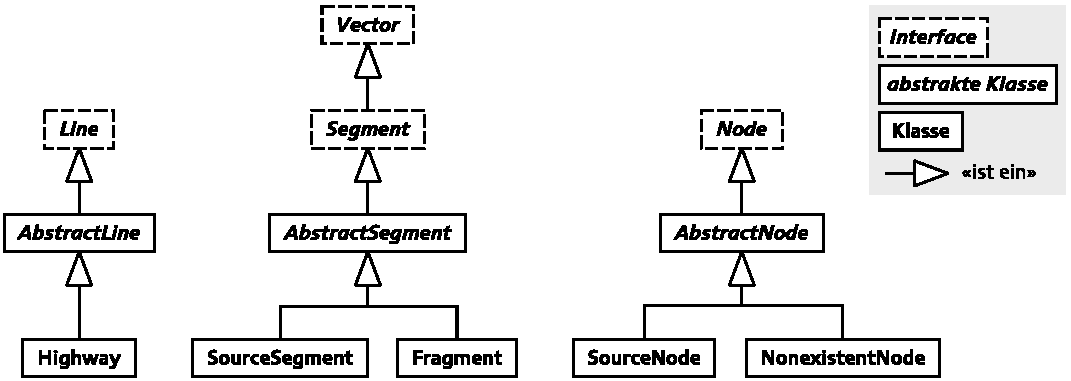
\includegraphics[scale=.8]{../chapter5/class-structure-splitting}
	\caption{Strukturdiagramm der für das \textproc{Splitten} relevanten Klassen}
	\label{fig:impl-class-structure-splitting}
}

Die Anzahl der jeweils das Interface implementierenden Klassen ist in diesem Projekt klein, so dass es sich anbietet, die jeweiligen Gemeinsamkeiten in abstrakten Klassen
% wie \code{AbstractSegment}
zusammenzufassen, um Redundanzen zu vermeiden.
Diese Klassen gehören daher zu den umfangreicheren im Projekt.
% Herauszustellen ist insbesondere die Klasse \code{AbstractSegment}, welche u.~a. wichtige Algorithmen wie \textproc{Fußpunkt} und \textproc{Analyse} enthält.

Wie in Abschnitt~\ref{ch:split-algorithm} erläutert, existiert derjenige \term{node}, an dem Segmente beim \textproc{Splitten} zerteilt werden, nicht in den Eingangsdaten.
Dementsprechend wird unterschieden zwischen \code{SourceNode} (aus den \osm-Quelldaten kommend) und \code{NonexistentNode} (beim \textproc{Splitten} entstehend).
Beide implementieren jedoch die gemeinsame Schnittstelle für den Typ \code{Node}.
Zu den Gemeinsamkeiten beider Arten von \code{Node}s gehören in erster Linie deren Koordinaten, welche folglich die Klasse \code{AbstractNode} verwaltet und an die beiden konkreten Implementierungen vererbt.

In gleicher Weise fasst \code{AbstractSegment} Gemeinsamkeiten solcher Segmente, die direkt aus den Eingangsdaten stammen (\code{SourceSegment}), und solcher Segmente, die erst durch \textproc{Splitten} eines anderen Segments entstehen (\code{Fragment}), zusammen.
In Abschnitt~\ref{ch:algorithm-parts} wurden solche Segmente zur Vereinfachung einander gleichgestellt.
Für derartige Fälle schlagen \citeauthor{GHJV95} den Einsatz des Kompositum-Entwurfsmusters vor:
„Use the Composite pattern when [...] you want clients to be able to ignore the difference between compositions of objects and individual objects. Clients will treat all objects in the composite structure uniformly.“ \citex[164]{GHJV95}
Im Kompositum-Muster werden Objekte zu Baumstrukturen aus individuellen Objekten (Blättern) und Komposita von Objekten zusammengefügt.

Im Kontext des Kompositum-Musters ist jedoch die Besonderheit zu berücksichtigen, dass hier einige Blätter aus den Eingangsdaten stammen (\code{SourceSegment}s), andere nicht (\code{Fragment}s).
Gleiches gilt auch für Komposita, so dass sich in einer nur auf Vererbung bestehenden Klassenstruktur sofort eine Wucherung aus größtenteils redundanten Klassen ergäbe.
Für solche Fälle schlagen \citeauthor{GHJV95} vor, das Brücken-Muster \term{(Bridge pattern)} einzusetzen, mit dem die Redundanz durch Delegation vermieden werden kann. \cf[153]{GHJV95}

\onefigure{ht}{
	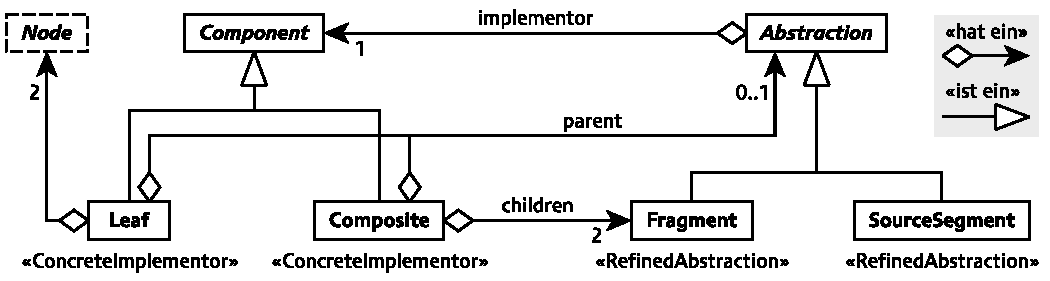
\includegraphics[scale=.8]{../chapter5/composite-bridge}
	\caption
		[Strukturdiagramm der Kombination aus \term{Composite} und \term{Bridge pattern}]
		{Strukturdiagramm einer Kombination aus \term{Composite pattern} und \term{Bridge pattern} \cf[153, 164]{GHJV95}}
	\label{fig:impl-composite-bridge}
}

Eine Kombination aus Kompositum und Brücke wäre zwar möglich, würde jedoch zu einer recht unübersichtlichen Struktur führen.
\Citeauthor{GHJV95} betonen, dass Delegation unweigerlich Komplexität mit sich bringt und nur dann sinnvoll ist, wenn andere Vorteile überwiegen („Delegation is a good design choice only when it simplifies more than it complicates.“ \citex[21]{GHJV95}).
Dies wäre hier offensichtlich nicht der Fall (Abbildung~\ref{fig:impl-composite-bridge}).

Ihre Empfehlung, Delegation möglichst nur in Form von standardisierten Mustern zu verwenden, [\cfibid] scheint hier auch wegen einer weiteren Besonderheit nicht anwendbar zu sein:
Alle Objekte im \code{AbstractSegment}-Kompositum sind veränderbar (\term{mutable}), damit bei der Umwandlung von Blättern (die jeweils ein Segment repräsentieren) in Komposita (die zwei oder mehr Segmente repräsentieren) beim \textproc{Splitten} keine großen Kosten entstehen.
Bloch betont die erheblichen Vorteile von \term{immutability} (\emph{nicht} veränderbarer Objekte), weist aber auch darauf hin, dass bestimmte komplexe Operationen dann sehr teuer werden können („The performance problem is magnified if you perform a multistep operation that generates a new object at every step, eventually discarding all objects except the final result.“ \citex[67]{Blo01}).
Im vorliegenden Kompositum würde \term{immutability} gerade erfordern, dass bei jedem \textproc{Splitten} der Baum neu aufgebaut wird.

Unterschiedliche Klassen für Blätter und Komposita sind deshalb hier nicht angebracht; vielmehr bietet es sich in Anlehnung an standardisierte Muster an, dass eine gemeinsame Klasse mit einem Attribut \term{children} sich entweder wie ein Blatt oder wie ein Kompositum verhält, je nachdem, ob es \term{children} in Form von Fragmenten gibt oder nicht.

\onefigure[13.5cm]{ht}{
	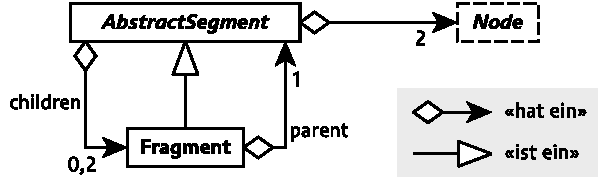
\includegraphics[scale=.8]{../chapter5/composite-actual}
	\caption{Diagramm der anstelle des \term{Composite pattern} gewählten vereinfachten Klassenstruktur für die beim \textproc{Splitten} entstehenden Fragmente}
	\label{fig:impl-class-structure-composite}
}

Aus dieser Erkenntnis ergibt sich eine vergleichsweise einfache Klassenstruktur (Abbildung~\ref{fig:impl-class-structure-composite}):
\code{AbstractSegment} implementiert die Gemeinsamkeiten aller Segmente.
Dazu gehört, dass jedes Segment in genau zwei Fragmente geteilt sein kann, die ihrerseits ebenfalls Segmente sind.
Jedes solche Fragment „weiß“ darüber hinaus, aus welchem Segment es abgetrennt wurde (\term{parent}).

%   [[ Textbausteine:
% In diesem speziellen Fall wird die Struktur der Komposition nur durch SPLITTEN verändert. Dabei wird genau ein Segment durch zwei andere ersetzt, die gemeinsam das ersetzte Segment repräsentieren.
% Dies entspricht zwar dem Composite-Leaf–Modell des Composite-Patterns, aber weil diese Unterscheidung orthogonal zur Unterscheidung in SourceSegment/Fragment ist, 
%   ]]

Die Unterschiede zwischen \code{SourceSegment} und \code{Fragment} sind zunächst klein.
Die in Abschnitt~\ref{ch:split-algorithm} gegebene Definition von \textproc{NaheSegmente} wurde über den schon erwähnten gepackten R-Baum in JTS implementiert.
Dessen Implementierung hat den Nachteil, dass der so erzeugte R-Baum nach dem Packen nicht mehr verändert werden darf.
\cf{jts:indexSTRtree}
% (im Gegensatz zu der Beschreibung in [RSV02 256]!)
Weil hier ohnehin \code{SourceSegment} als eigene Klasse existiert, bietet es sich an, die \textproc{NaheSegmente}-Logik nur in \code{SourceSegment} zu implementieren statt in der Superklasse \code{AbstractSegment}.
Das Packen des R-Baums braucht dann nur genau einmal nach dem Segmentieren durchgeführt zu werden.
Danach werden die \code{SourceSegment}s nicht mehr verändert.
Da Abschnitt~\ref{ch:split-algorithm} ohnehin eine erneute Abstandsprüfung in der späteren \textproc{Analyse} vorsieht, stellt diese Abweichung von der Definition der Algorithmen nicht die Korrektheit der Implementierung in Frage, obwohl sie mehr Segmente als „nah“ betrachtet als die formale Beschreibung für \textproc{NaheSegmente}.
% (weil SourceSegments obdA größer als Fragments sind). (aber NAHESEGMENTE ist ja primär eine Optimierung)

% TODO:
% Vector erwähnen!

% (weitere Besonderheiten der Konkreten ggü. Abstract*?)
%- SourceNode enthält neben der ID nur Pointers zu den Segmenten etc. für die Korralation
%- SourceSegment außerdem nur L+R sowie analyseLineParts



\subsection{Analyse und Anwendbarkeit auf andere Spezialfälle}
\label{ch:impl-analyser}

Die Algorithmen zur \textproc{Analyse} erfordern die Ergänzung des Datenmodells aus Abbildung~\ref{fig:impl-geometry-model} mit den zusätzlichen Attributen $\relation{parallelLinks}$ und $\relation{parallelRechts}$, in denen das Ergebnis der \textproc{Analyse} abgelegt wird.
Wie in Abschnitt~\ref{ch:algorithm-parts} definiert sind dies Attribute des Wurzel-Segments, also der Klasse \code{SourceSegment}.

Obwohl nach der Auswahl eines bestimmten Spezialfalls der Liniengeneralisierung in Abschnitt~\ref{ch:case-selection} andere Fälle nicht weiter berücksichtigt wurden, ist eine auch andere Anwendungsfälle zulassende Flexibilität doch Teil der angestrebten Praxistauglichkeit der zu entwickelnden Software.
Angesichts der Arbeitsweise der Algorithmen ist es naheliegend, dass sich dies insbesondere in der Analyse auf Parallelität niederschlagen sollte.
Die Definition der \textproc{Analyse} beschränkt sich auf geometrische Aspekte; für die konkrete Evaluierung zweiter Segmente spielen im Wesentlichen die Definitionen für \textproc{Parallel} und \textproc{Distanz} eine Rolle.
Es wäre daher von Vorteil, wenn diese beiden Definitionen in der Software leicht austauschbar wären.

Dieses Verhalten scheint auf den ersten Blick auf die Beschreibung des Schablonenmethoden"=Entwurfsmusters \term{(Template Method pattern)} zu passen, womit einzelne Schritte verändert werden können, ohne die gesamte Struktur eines Algorithmus zu verändern.
Tatsächlich beschränkt sich dieses Muster jedoch darauf, diese einzelnen Schritte von Unterklassen implementieren zu lassen, was auch in der einleitenden Beschreibung von \citeauthor{GHJV95} schon deutlich wird:
„Template Method lets subclasses redefine certain steps of an algorithm without changing the algorithm's structure.“ \citex[325]{GHJV95}
Eine Anwendung an dieser Stelle würde also gerade unter Berücksichtigung der oben beschriebenen Komposition von Segmenten in \code{SourceSegment}s und \code{Fragment}s zu einer Wucherung von weiteren Unterklassen führen und wäre daher ungeeignet.

Stattdessen empfehlen \citeauthor{GHJV95} das Besucher-Muster \term{(Visitor pattern)} einerseits gerade für solche Kompositionen, andererseits gerade dann, wenn wie hier die eigentlichen Datenstrukturen stabil sind, aber doch Flexibilität zur Definition neuer Operationen bieten sollen. \cf[333, 344]{GHJV95}
Dabei erlauben die Objekte der bereits etablierten Datentypen, ihnen einen sog. \term{visitor} als ein unabhängiges Objekt mit definierter Schnittstelle zu übergeben, welches die jeweiligen Operationen implementiert. \cf[331--335]{GHJV95}

In der vorliegenden Software akzeptieren die Segmente den Besuch eines Objekts, das die Schnittstelle \code{Analyser} implementiert.
Dieses Objekt soll die Implementierungen der Algorithmen \textproc{Parallel} und \textproc{Distanz} enthalten.
Im Sinne der besprochenen Systemarchitektur braucht somit das Wissen über das Behandeln des in Abschnitt~\ref{ch:case-selection} gewählten Spezialfalls „baulich getrennte Richtungsfahrbahnen im Straßenraum“ nicht Teil des \term{Combiners} zu sein, sondern kann vom Client auf andere Themen angepasst werden.



\subsection{Punktezuordnung}
\label{ch:impl-node-match}

Für Abschnitt~\ref{ch:node-match-algorithm} ergibt sich das in Abbildung~\ref{fig:impl-node-match-model} gezeigte Datenmodell.
Die Klasse \code{NodeMatch} implementiert die Punktezuordnungen.
Dies sind entsprechend der formalen Definition Mengen aus exakt zwei gegenüberliegenden \term{nodes} einander paralleler Segmente.
Die Definition als mathematische Menge zur Vermeidung von Duplikaten wird später beim Zusammenfassen die Interpretation des Begriffs „nächste Zuordnung $Z'$“ erleichtern (vergleiche Abschnitt~\ref{ch:generalisation-algorithm}).
Um Objekte der Klasse \code{NodeMatch} klar als Menge zu kennzeichnen, wurde sie zusätzlich als \code{Set<Node>} (Menge von \code{Node}s) im Java Collections Framework deklariert.
Dies erleichtert auch die Implementierung der Mengeneigenschaften.

\onefigure{ht}{
% [NodeGraph]1 <>-- 1…n[NodeMatch]0…n <>-- 2[Node]
	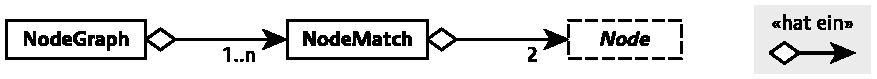
\includegraphics[scale=.8]{../chapter5/model-node-match}
	\caption{Datenmodell für die Punktezuordnung}
	\label{fig:impl-node-match-model}
}

Da die \textproc{Analyse} für jedes Segment immer jeweils links- und rechtsseitig nach Parallelen sucht, werden beim \textproc{NodesZuordnen} viele Zuordnungen doppelt gefunden, nämlich einmal in jeder Richtung.
Erneut vereinfachen die Eigenschaften der mathematischen Menge, hier der Menge aller Zuordnungen $\mathcal{Z}$, die Beschreibung des Algorithmus in Abschnitt~\ref{ch:node-match-algorithm}.
Weil \code{NodeMatch}-Objekte wie beschrieben die Mengeneigenschaften implementieren, können sie leicht direkt im Java Collections Framework verwendet werden, hier als \code{Set<NodeMatch>} (Menge von \code{NodeMatch}-Objekten).
Da der Datentyp \code{NodeMatch} gleichzeitig die Schnittstelle \code{Set<Node>} implementiert, hat die Menge aller Zuordnungen implizit den Typ \code{Set<Set<Node>>}, ist also eine Menge \emph{von Mengen} von \term{nodes}, was genau der formalen Anforderung in Abschnitt~\ref{ch:node-match-algorithm} entspricht.

Punktezuordnungen und Segmente ergeben gemeinsam einen gemischten Graphen des zu generalisierenden Netzes.
Als parallel erkannte Segmente sind über deren \term{nodes} derart einander zugeordnet, dass sich eine gemeinsame Mittellinie als Verknüpfung der Mittelpunkte derjenigen Kanten im Graphen, welche die Punktezuordnungen darstellen, leicht finden lässt.
Zur Definition des Graphen genügt die Menge aller Punktezuordnungen, wenn über die einzelnen Punkte die mit ihnen verknüpften Segmente ermittelbar sind.

% TODO: ist hier der Fall, über addSegment(), welches in AbstractLine passiert. Sollte vielleicht weiter oben in 4.3.1 erwähnt werden. Eventuell könnte auch eine Grafik eines solchen Graphen nicht schaden.



\subsection{Liniengeneralisierung}
\label{ch:impl-generalisation}

Das Ergebnis der Liniengeneralisierung nach Abschnitt~\ref{ch:generalisation-algorithm} ist ein Graph aus Linienzügen, von denen einige durch Zusammenfassen entstehen, andere jedoch mangels Parallelen direkt aus den Eingangsdaten übernommen werden.
Der beschriebene Algorithmus zum \textproc{Zusammenfassen} ergibt einzelne Segmente.
Um die spätere Weiterverarbeitung des Generalisierungsergebnisses zu erleichtern, werden sowohl diese als auch Segmente ohne Parallele zu möglichst langen Linienzügen verkettet.

\onefigure{ht}{
% [GeneralisedLines]1 <>-- 0…n[ResultLine (Section/GeneralisedSection)]0…n <>-- 2…n[Node]
	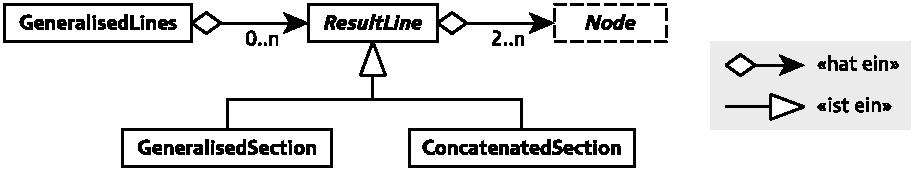
\includegraphics[scale=.8]{../chapter5/model-generalisation}
	\caption{Datenmodell für das Zusammenfassen}
	\label{fig:impl-generalisation-model}
}

Entsprechend gibt es zwei unterschiedliche Arten von Linienzügen in den Ergebnisdaten.
Dies wird auch vom Datenmodell so abgebildet (Abbildung~\ref{fig:impl-generalisation-model}).
Die Klassen \code{GeneralisedSection} und \code{ConcatenatedSection} enthalten jeweils im Konstruktor Code, der allein anhand der Angabe eines geeigneten Startpunkts einen Linienzug für das Ergebnis bildet.
Die bearbeiteten Segmente werden dabei entsprechend markiert, um doppelte Bearbeitungen zu vermeiden.

Die Klasse \code{GeneralisedSection} enthält den Algorithmus zum \textproc{Zusammenfassen}.
\code{ConcatenatedSection} ist ähnlich aufgebaut, aber wesentlich einfacher, da Punktezuordnungen keine Rolle spielen, sondern nur die jeweils anschließenden Segmente zu berücksichtigen sind.
Beide Klassen sind vom Typ \code{ResultLine}, um dem Client des \term{Combiners} einen einheitlichen Typ für die Ergebnisdaten liefern zu können.

Die Klasse \code{GeneralisedLines} ist eine einfache Fassade für die Generalisierung, um deren Einsatz zu erleichtern.
\cf[186]{GHJV95}



% Given unlimited time, I might continue working on this for a long time … but I think what has already been written is enough detail for the intended audience, especially considering that the API documentation is also available.

%\subsection{Integration und ggf. Datenfluss/Interaktionswege \emph{[ausstehend]}}
%
%\begin{itemize}
%\item Integration der beschriebenen Klassen zu einem funktionierenden System
%\item \code{Combiner} = Façade
%\item ggf. Datenfluss/Interaktionswege
%% (weichen im imperativen Code teils deutlich von funktional formulierten Algorithmen ab)
%\end{itemize}



\section{Schwierigkeiten bei der Umsetzung}
\label{ch:impl-difficulties}

Im Laufe der Implementierung ergaben sich nicht vorhergesehene Probleme und Erkenntnisse.
In den folgenden Abschnitten werden diese kurz erläutert.



\subsection{Eigenschaften der Sprache}

Die Entwicklung von der Idee für einen Algorithmus hin zu einer für komplexe Geodaten praxistauglichen Implementierung kann als iterativer Prozess verstanden werden:
Unter dem Eindruck der Ergebnisse früher Versionen werden Algorithmus und Implementierung nach und nach verfeinert.
% http://de.wikipedia.org/wiki/Prototyping_(Softwareentwicklung)#Evolution.C3.A4res_Prototyping
Die Wahl von Java als streng typisierte Sprache erschwerte jedoch dieses Vorgehen.
%Der Zeitaufwand dafür, elegante Klassenstrukturen aufzubauen, wurde vom Verfasser unterschätzt.
Die strenge Typisierung hat den Fokus dieser Arbeit (unter Berücksichtigung des vorgegebenen Umfangs notwendigerweise) ein Stück weit verschoben von Algorithmusentwicklung und -beurteilung zu den Details objektorientierter Programmierung.
Dies war so vor Beginn nicht absehbar.
% denn nur ich+Jochen waren Programmierer, aber nur die offiziellen Betreuer haben akad. Erfahrung

Möglicherweise wäre eine dynamisch typisierte Skriptsprache wie Perl für dieses explorative Vorgehen geeigneter gewesen.
Den vermuteten Effizienznachteilen solcher Sprachen (siehe Abschnitt~\ref{ch:impl-env}) steht die einfachere Umsetzung von Änderungen gegenüber.

Weiterhin war das Aufbauen eigener Datenstrukturen für die Arbeit mit Segmenten lehrreich, aber zeitaufwändiger als erwartet.
Erwartungsgemäß war dabei jedoch das Java Collections Framework äußerst hilfreich.

Ebenfalls als hilfreich stellte sich die Idee heraus, nicht nur im Algorithmus (Abschnitt~\ref{ch:split-algorithm}), sondern auch in der Typenhierarchie Segmente als Vektoren zu behandeln.
Die Implementierung des \term{Combiners} setzt dies um, indem über Interface-Vererbung alle Segmente auch Vektoren sind (siehe Abbildung~\ref{fig:impl-class-structure-splitting}).
Es ist denkbar, dass eine Sprache mit Operatorüberladung wie Perl dies noch eleganter hätte lösen können.



\subsection{Ein- und Ausgabe von Geodaten}
\label{ch:impl-io}

Im Zuge der Entwicklung stellte sich schnell heraus, dass die direkte Verwendung von \osm-Daten etwas schwieriger war als erwartet.
Die Eingabe wurde daher zunächst über die unter \href{https://download.geofabrik.de/}{\nolinkurl{download.geofabrik.de}} angebotenen \osm-Shapefiles realisiert.
% ein spezielles Shapefile, das zusätzlich die OSM-IDs der Start- und End-Nodes enthält (nur als Debugging-Hilfe; die Algorithmen sind nicht davon abhängig)
Auch die Ausgabe erfolgt zunächst als Shapefile, damit das Generalisierungsergbnis leicht mit gängiger Software betrachtet werden kann.

Die Shapefiles der Geofabrik enthalten aus technischen Gründen veränderte Attribute anstelle der Original-\osm-\term{tags}.
Diesem Problem wurde begegnet, indem ein Adapter (\term{object adapter} \cf[139--141]{GHJV95}) die aus den Shapefiles gelesenen Attribute wieder zurück in das \osm-Format wandelt, ohne dass dies für den \term{Combiner} sichtbar wird.
% Adapter pattern: io.ShapeGeofabrikAdapter

Die Nutzung des \term{frameworks} GeoTools zur Ein- und Ausgabe von Geodaten war unerwartet problematisch.
Zwar bietet GeoTools umfangreiche Unterstützung für verschiedene Datenformate, jedoch sind die entsprechenden GeoTools-Klassen umständlich zu benutzen, ihr Interface ist nicht stabil und sie arbeiten sehr langsam.
Es ist gelungen -- wenn auch mit erheblichem Zeitaufwand --, eine Lösung hierfür zu entwickeln.

Um die Datenausgabe auf eine akzeptable Geschwindigkeit zu beschleunigen, werden diese nun im GeoJSON-Format ausgegeben (implementiert als reine Textausgabe, was sehr billig ist).
Das GeoJSON wird anschließend mit GDAL in ein Shapefile konvertiert.
Insgesamt ist diese Lösung um ein Vielfaches schneller als die von GeoTools zur Verfügung gestellte Shapefile-Ausgabe.%
\footnote{In der später erschienenen Version 10.0 von GeoTools ist die Shapefile-Unterstützung neu implementiert. \cf{Deo13} Dem ersten Anschein nach löst dies die beschriebenen Probleme nicht.}
% http://web.archive.org/web/20130926213903/http://docs.codehaus.org/display/GEOTOOLS/Migrate+shapefile+to+shapefile-ng

Außer dem eigentlichen Generalisierungsergebnis kann der \term{Combiner} auch zahlreiche zusätzliche Geodatensätze ausgeben, die das Verständnis von der Arbeitsweise des Algorithmus bei Anwendung auf \term{real world}--Daten verbessern und auch bei der Fehlersuche hilfreich sind.
Diese Ausgaben sind in keiner Weise optimiert.
Sie können mit dem Schalter \texttt{--debug} kontrolliert werden.



\subsection{Flexibilität und Effizienz}
\label{ch:impl-flexibility-efficiency}

Die Definition des Spezialfalls, auf den die Arbeit beschränkt werden soll, in einem eigenen Paket \code{highway} vom Rest des Combiners zu trennen und sie damit leicht austauschbar zu machen, war grundsätzlich eine gute Idee.
Eine solche Trennung konsequent umzusetzen, wäre allerdings über die Aufgabenstellung hinaus gegangen.
%Diese Trennung ist allerdings bisher nur begonnen worden und konnte aus Zeitgründen nicht bis zum Abschluss der Arbeit beendet werden; angesichts der ausdrücklichen Beschränkung in der Aufgabenstellung auf nur den ausgewählten Spezialfall war das aber auch streng genommen gar nicht notwendig.
% betrifft insb. die Klassen Line, AbstractLine, io.InputDataset, io.ShapeReader sowie GeneralisedSection/Section

Im Unterschied zur formalen Definition in Abschnitt~\ref{ch:analyse-algorithm} sind $\relation{parallelLinks}$ und $\relation{parallelRechts}$ nicht als homogene binäre Relation auf Segmenten implementiert, sondern als Relation zwischen Segmenten und \emph{Mengen} von Segmenten.
Mit anderen Worten: Es wird nicht jeweils nur ein einziges Segment je Seite als „parallel“ markiert, sondern mehrere.
% es wird in der Tat wie theoretisch überlegt durch die reziproke Zuordnung sichergestellt, dass auch ohne Liste für jedes Paar eine Zuordnung erstellt wird
Auf die Korrektheit der Algorithmen hat dies keinen Einfluss.
Zwar entstehen beim \textproc{NodesZuordnen} zunächst mehr Zuordnungen.
Dies sind jedoch Duplikate, die aufgrund der Mengeneigenschaft entfallen (vergleiche Abschnitt~\ref{ch:impl-node-match}).
Es stellt sich hier also die Frage, welche Implementierungsvariante mit dem Java Collections Framework am effizientesten umzusetzen ist.
Ein \term{profiling} wurde noch nicht durchgeführt.
% => Optimierungspotenzial

Eine besonders effiziente Implementierung stand nicht im Vordergrund.
Die gewählten Datenstrukturen haben einen höheren Speicherbedarf als eigentlich nötig.
Beispielsweise werden in den Implementierungen der Algorithmen \textproc{Fußpunkt} (verwendet beim \textproc{Splitten} von Segmenten) und \textproc{Analyse} zahlreiche neue Vektoren-Objekte erzeugt, die jeweils nur für eine einzige geometrische Berechnung benötigt werden.
% in 6.4 wird insbesondere das SPLITTEN diskutiert; das sollte hier erwähnt werden!
Die dadurch häufiger notwendige automatische Freispeichersammlung \term{(garbage collection)} zur Beseitigung dieser Objekte ist zeitaufwändig.
Diese Zeit- und Speicherkosten hängen von der gewählten Implementierung ab und konnten deshalb in Abschnitt~\ref{ch:algorithm-overview} nicht berücksichtigt werden.
Insbesondere für den Speicheraufwand besteht Optimierungspotenzial.

% https://docs.oracle.com/javase/7/docs/api/java/lang/ref/WeakReference.html

Ohnehin musste die Software aus Zeitgründen ohne besondere Rücksicht auf die Eigenschaften von Compiler und Hardware entwickelt werden.
Speicherzugriff und -verwaltung sind deshalb wahrscheinlich erhebliche Engpässe des \term{Combiners.}

Ein Beispiel für unnötigen Speicheraufwand ist die Bildung durchgehender Linienzüge im Generalisierungsergebnis:
Diese sind in Kapitel~\ref{ch:algorithm-parts} spezifiziert als Mengen zusammenhängender Segmente und sind auch so in \code{AbstractLine} implementiert.
Tatsächlich müssen diese Segmente jedoch für \code{AbstractLine} in jedem Fall erst anhand einer Liste von Stützpunkten erzeugt werden.
Da für \code{ResultLine} die Segmente später ohnehin nur benötigt werden, um daraus gerade eine Liste von Stützpunkten zu erzeugen, wäre eine Optimierung von \code{AbstractLine} durch \term{lazy initialisation} angebracht:
Es würde in \code{AbstractLine} zunächst die Liste von \term{nodes} gespeichert und die Segmentierung nur dann durchgeführt, wenn tatsächlich \textproc{Segmente} angefordert werden.
% Oder es könnte evtl. auch recht einfach ResultLine einige Methoden überschreiben (coordinates, add (-> protected), get/size/iterator etc.)



% single-chapter commands
\onlyinsubfile{\listoffigures}
\onlyinsubfile{\subfile{../bibliography/Literaturverzeichnis}}
\end{document}
